\documentclass[a4paper,oneside,DIV=10,12pt]{scrartcl}

\usepackage{float}

\usepackage{fontspec}
\setmainfont{STIX Two Text}
\setsansfont{Roboto}
%\newfontfamily{\cyrillicfontsf}{Raleway}
\setmonofont{PT Mono}

\usepackage{microtype}

\usepackage{amsmath}
\usepackage{unicode-math}
\setmathfont{STIX Two Math}

\usepackage{polyglossia}
\setmainlanguage{ukrainian}

\usepackage{graphicx}

\usepackage{booktabs}

\usepackage{subcaption}

\usepackage{siunitx}
\sisetup{output-decimal-marker = {,}}

\newcommand\schel[1]{\textit{#1}}

\begin{document}
	\begin{titlepage}
	\begin{center}
		Міністерство освіти і науки України\\
		Національний авіаційний університет\\
		Навчально-науковий інститут комп'ютерних інформаційних технологій\\
		Кафедра комп'ютеризованих систем управління

		\vspace{\fill}
		Лабораторна робота №3\\
		з дисципліни «Комп'ютерна електроніка»\\
		на тему «Дослідження біполярного транзистора у~ключовому режимі для~схеми с загальним емітером»\\
		Варіант №3
		
		\vspace{\fill}
		\begin{flushright}
		Виконав:\\
		студент ННІКІТ СП-225\\
		Клокун Владислав\\
		Перевірив:\\
		Андрєєв О. В.
		\end{flushright}
		
		Київ 2017
	\end{center}
	\end{titlepage}
	
	\section{Мета та основні завдання роботи}
		\begin{enumerate}
			\item Закріпити теоретичні знання з фізики процесів, що відбуваються в біполярному тразисторі, який працює в ключовому режимі.
			\item Набути практичних навичок у визначенні основних параметрів перехідних процесів.
			\item Вивчити процеси,  що відбуваються у біполярному транзисторі у ключовому режимі.
			\item Вивчити, від чого залежить час увімкнення й вимкнення біполярного транзистора.
		\end{enumerate}
	
	\section{Принципова схема віртуальної лабораторної установки}
		Принципова схема віртуальної лабораторної установки для дослідження біполярного транзистора у ключовому режимі зображена на рис. \ref{fig:schematic}.
		\begin{figure}[H]
			\centering
			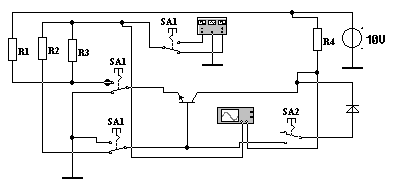
\includegraphics[width=\textwidth]{lab-03-01-schematic.png}
			\caption{Принципова схема віртуальної лабораторної установки}
			\label{fig:schematic}
		\end{figure}
		
	\section{Хід роботи}
		%Готуємо віртуальну лабораторну установку до роботи.
		Вмикаємо біполярний транзистор за схемою з загальним емітером. Для цього встановлюємо перемикач \schel{SA1} в нижнє положення. Відключаємо діод, встановивши перемикач \schel{SA2} у верхнє положення. Вмикаємо осцилограф та встановлюємо на ньому такі режими і масштаби:
		\begin{table}[H]
		\centering
			\begin{tabular}{lll}
			Time Base & 0,2 μs/div & Y/T; Auto\\
			Channel A & 2 V/div & DC \\
			Channel B & 5 V/div & DC
			\end{tabular}
		\end{table}
		
		Вмикаємо функціональний генератор та налаштовуємо його на генерацію прямокутних імпульсів. Встановлюємо такі налаштування:
		\begin{table}[H]
		\centering
			\begin{tabular}{ll}
			Frequency & 1 MHz\\
			Duty cycle & 50\%\\
			Amplitude & 1,5 V
			\end{tabular}
		\end{table}
		
		Запускаємо віртуальну установку на моделювання. На екрані осцилографа з'я\-ви\-лась часова діаграма вхідної і вихідної напруг транзистора. Призупиняємо моделювання і вимірюємо амплітуди вхідного імпульсу: $U_{\text{Б}} = \SI{1,5}{\volt}$ та вихідного імпульсу: $U_{\text{К}} = \SI{10}{\volt}$. Амплітуда вихідного імпульсу близька за значенням до напруги $E_{\text{К}} = \SI{10}{\volt}$, отже транзистор знаходиться в \emph{режимі насичення}.
		
		За допомогою візирних ліній визначаємо часові параметри з діодом і без.
		
		%$t_{\text{ЗТ}} = \SI{2,5}{\nano\second}$, $t_{\text{НР}} = \SI{11,8}{\nano\second}$, $t_{\text{Р}} = \SI{3,6}{\nano\second}$, $t_{\text{СП}} = \SI{7,6}{\nano\second}$.
		
		\begin{table}[H]
		\centering
			\begin{subtable}[h]{0.4\textwidth}
			\centering
				\begin{tabular}{lr}
				\toprule
				Параметр & Значення\\
				\midrule
				$t_{\text{ЗТ}}$ & $\SI{2,5}{\nano\second}$\\
				$t_{\text{НР}}$ & $\SI{11,8}{\nano\second}$\\
				$t_{\text{Р}}$ & $\SI{3,6}{\nano\second}$\\
				$t_{\text{СП}}$ & $\SI{7,6}{\nano\second}$\\
				\bottomrule
				\end{tabular}
				\caption{З вимкненим діодом}
			\end{subtable}
			~
			\begin{subtable}[h]{0.4\textwidth}
			\centering
				\begin{tabular}{lr}
				\toprule
				Параметр & Значення\\
				\midrule
				$t_{\text{ЗТ}}$ & $\SI{0}{\nano\second}$\\
				$t_{\text{НР}}$ & $\SI{91}{\nano\second}$\\
				$t_{\text{Р}}$ & $\SI{125}{\nano\second}$\\
				$t_{\text{СП}}$ & $\SI{64}{\nano\second}$\\
				\bottomrule
				\end{tabular}
				\caption{З ввімкненим діодом}
			\end{subtable}
			
		\caption{Часові параметри біполярного транзистора, підключеного за схемою с загальним емітером при $U_{\text{Е}} = \SI{1,5}{\volt}$}
		\end{table}
		
		За отриманими часовими параметрами рахуємо $t_{\text{ВВІМК}}$ і $t_{\text{ВИМК}}$:
		\[
			t_{\text{ВВІМК}} = t_{\text{ЗТ}} + t_{\text{НР}} = \SI{14,3}{\nano\second}, \quad t_{\text{ВИМК}} = t_{\text{Р}} + t_{\text{СП}} = \SI{11,2}{\nano\second}.
		\]
		
		Для ввімкненого діода:
		\[
			t_{\text{ВВІМК}} = t_{\text{ЗТ}} + t_{\text{НР}} = \SI{91}{\nano\second}, \quad t_{\text{ВИМК}} = t_{\text{Р}} + t_{\text{СП}} = \SI{189}{\nano\second}.
		\]
		
		%\[
		%	t_{\text{ВИМК}} = t_{\text{Р}} + t_{\text{СП}} = \SI{3,6}{\nano\second} + \SI{7,6}{\nano\second} = \SI{11,2}{\nano\second}.
		%\]
		
		\begin{figure}[H]
		\label{fig:u1p5nodiode}
		\centering
			\def\svgwidth{\columnwidth}
			\input{1p5v-nodiode.pdf_tex}
		\caption{Часова діаграма вхідної і вихідної напруг для $U_{\text{Е}} = \SI{1,5}{\volt}$ з вимкненим діодом}
		\end{figure}
		
		\begin{figure}[H]
		\label{fig:u1p5diode}
		\centering
			\def\svgwidth{\columnwidth}
			\input{1p5v-diode.pdf_tex}
		\caption{Часова діаграма вхідної і вихідної напруг для $U_{\text{Е}} = \SI{1,5}{\volt}$ з ввімкненим діодом}
		\end{figure}
		
		\newpage
		
		Відключаємо діод. На функціональному генераторі встановлюємо амплітуду вхідних імпульсів рівну $U_{\text{ВХ}} = \SI{0,7}{\volt}$. При цьому амплітуда вихідних імпульсів зменшилась. Біполярний транзистор знаходиться в \emph{активному режимі}. За допомогою візирних ліній визначаємо часові параметри.
		
		\begin{table}[H]
		\centering
			\begin{subtable}[h]{0.4\textwidth}
			\centering
				\begin{tabular}{lr}
				\toprule
				Параметр & Значення\\
				\midrule
				$t_{\text{ЗТ}}$ & $\SI{7,8}{\nano\second}$\\
				$t_{\text{НР}}$ & $\SI{115}{\nano\second}$\\
				$t_{\text{Р}}$ & $\SI{0}{\nano\second}$\\
				$t_{\text{СП}}$ & $\SI{5}{\nano\second}$\\
				\bottomrule
				\end{tabular}
				\caption{З вимкненим діодом}
			\end{subtable}
			~
			\begin{subtable}[h]{0.4\textwidth}
			\centering
				\begin{tabular}{lr}
				\toprule
				Параметр & Значення\\
				\midrule
				$t_{\text{ЗТ}}$ & $\SI{0}{\nano\second}$\\
				$t_{\text{НР}}$ & $\SI{377}{\nano\second}$\\
				$t_{\text{Р}}$ & $\SI{1}{\nano\second}$\\
				$t_{\text{СП}}$ & $\SI{20}{\nano\second}$\\
				\bottomrule
				\end{tabular}
				\caption{З ввімкненим діодом}
			\end{subtable}
			
		\caption{Часові параметри біполярного транзистора, підключеного за схемою с загальним емітером при $U_{\text{Е}} = \SI{0,7}{\volt}$}
		\end{table}
		
		За отриманими часовими параметрами рахуємо $t_{\text{ВВІМК}}$ і $t_{\text{ВИМК}}$:
		\[
			t_{\text{ВВІМК}} = t_{\text{ЗТ}} + t_{\text{НР}} = \SI{115}{\nano\second}, \quad t_{\text{ВИМК}} = t_{\text{Р}} + t_{\text{СП}} = \SI{5}{\nano\second}.
		\]
		
		Для ввімкненого діода:
		\[
			t_{\text{ВВІМК}} = t_{\text{ЗТ}} + t_{\text{НР}} = \SI{377}{\nano\second}, \quad t_{\text{ВИМК}} = t_{\text{Р}} + t_{\text{СП}} = \SI{20}{\nano\second}.
		\]
		
		\begin{figure}[H]
		\label{fig:u0p7nodiode}
		\centering
			\def\svgwidth{\columnwidth}
			\input{0p7v-nodiode-edited.pdf_tex}
		\caption{Часова діаграма вхідної і вихідної напруг для $U_{\text{Е}} = \SI{0,7}{\volt}$ з вимкненим діодом}
		\end{figure}
		
		%Підключаємо діод і визначаємо часові параметри: $t_{\text{ЗТ}} = \SI{0}{\nano\second}$, $t_{\text{НР}} = \SI{377}{\nano\second}$, $t_{\text{0}} = \SI{0}{\nano\second}$, $t_{\text{СП}} = \SI{20}{\nano\second}$.
		
		\begin{figure}[H]
		\label{fig:u0p7diode}
		\centering
			\def\svgwidth{\columnwidth}
			\input{0p7v-diode-edited.pdf_tex}
		\caption{Часова діаграма вхідної і вихідної напруг для $U_{\text{Е}} = \SI{0,7}{\volt}$ з ввімкненим діодом}
		\end{figure}
		
		%\newpage
		
		Відключаємо діод. На функціональному генераторі встановлюємо амплітуду вхідних імпульсів рівну $U_{\text{ВХ}} = \SI{2,3}{\volt}$. При цьому збільшились амплітуда вихідних імпульсів і час $t_{\text{Р}}$. Біполярний транзистор знаходиться в \emph{режимі глибокого насичення}. Визначаємо часові параметри з вимкненим і ввімкненим діодом.
		%$t_{\text{ЗТ}} = \SI{0}{\nano\second}$, $t_{\text{НР}} = \SI{26}{\nano\second}$, $t_{\text{Р}} = \SI{5}{\nano\second}$, $t_{\text{СП}} = \SI{5}{\nano\second}$.
		
		\begin{table}[H]
		\centering
			\begin{subtable}[h]{0.4\textwidth}
			\centering
				\begin{tabular}{lr}
				\toprule
				Параметр & Значення\\
				\midrule
				$t_{\text{ЗТ}}$ & $\SI{0}{\nano\second}$\\
				$t_{\text{НР}}$ & $\SI{26}{\nano\second}$\\
				$t_{\text{Р}}$ & $\SI{5}{\nano\second}$\\
				$t_{\text{СП}}$ & $\SI{5}{\nano\second}$\\
				\bottomrule
				\end{tabular}
				\caption{З вимкненим діодом}
			\end{subtable}
			~
			\begin{subtable}[h]{0.4\textwidth}
			\centering
				\begin{tabular}{lr}
				\toprule
				Параметр & Значення\\
				\midrule
				$t_{\text{ЗТ}}$ & $\SI{0}{\nano\second}$\\
				$t_{\text{НР}}$ & $\SI{46}{\nano\second}$\\
				$t_{\text{Р}}$ & $\SI{216}{\nano\second}$\\
				$t_{\text{СП}}$ & $\SI{81}{\nano\second}$\\
				\bottomrule
				\end{tabular}
				\caption{З ввімкненим діодом}
			\end{subtable}
			
		\caption{Часові параметри біполярного транзистора, підключеного за схемою с загальним емітером при $U_{\text{Е}} = \SI{2,3}{\volt}$}
		\end{table}
		
		За отриманими часовими параметрами рахуємо $t_{\text{ВВІМК}}$ і $t_{\text{ВИМК}}$:
		\[
			t_{\text{ВВІМК}} = t_{\text{ЗТ}} + t_{\text{НР}} = \SI{115}{\nano\second}, \quad t_{\text{ВИМК}} = t_{\text{Р}} + t_{\text{СП}} = \SI{5}{\nano\second}.
		\]
		
		Для ввімкненого діода:
		\[
			t_{\text{ВВІМК}} = t_{\text{ЗТ}} + t_{\text{НР}} = \SI{46}{\nano\second}, \quad t_{\text{ВИМК}} = t_{\text{Р}} + t_{\text{СП}} = \SI{397}{\nano\second}.
		\]
		
		\begin{figure}[H]
		\label{fig:u2p3nodiode}
		\centering
			\def\svgwidth{\columnwidth}
			\input{2p3v-nodiode-edited.pdf_tex}
		\caption{Часова діаграма вхідної і вихідної напруг для $U_{\text{Е}} = \SI{2,3}{\volt}$ з вимкненим діодом}
		\end{figure}
		
		%Підключаємо діод і визначаємо часові параметри: $t_{\text{ЗТ}} = \SI{0}{\nano\second}$, $t_{\text{НР}} = \SI{46}{\nano\second}$, $t_{\text{Р}} = \SI{216}{\nano\second}$, $t_{\text{СП}} = \SI{81}{\nano\second}$.
		
		\begin{figure}[H]
		\label{fig:u2p3diode}
		\centering
			\def\svgwidth{\columnwidth}
			\input{2p3v-diode-edited.pdf_tex}
		\caption{Часова діаграма вхідної і вихідної напруг для $U_{\text{Е}} = \SI{2,3}{\volt}$ з ввімкненим діодом}
		\end{figure}
		
	\section{Висновки}
		Виконуючи дану лабораторну роботу, вдалось визначити за експериментальними даними, що при ввімкнені біполярного транзистора у схемі з загальним емітером, він найшвидше перемикається в режимі насичення з вимкненим діодом: $t_{\text{ВВІМК}} + t_{\text{ВИМК}} = \SI{25,5}{\nano\second}$.
\end{document}
